\subsection{Completion, Deadlines and Paired Rollout Sensitivity}
\label{app:completion-sensitivity}

These analyses reuse the 45 equal-cap queries and their two stored rollouts. They add no independent cases or model calls. All-case correctness keeps failed and invalid outputs in the denominator. Let $S$ be the queries for which every route returns a valid answer within 1,200 seconds. The selected comparison $|S|^{-1}\sum_{i\in S}(Y_{ir}-Y_{is})$ changes both the numerator and denominator. It is descriptive and cannot estimate what would have happened had an incomplete execution succeeded.

\begin{table}[htbp]
\centering
\small
\begin{tabular}{@{}llrrr@{}}
\toprule
Rollout & RLM minus & All 45 & Common completions & Change \\
\midrule
Seed 20 ($|S|=39$) & Iterative & $-4.4$ & $+5.1$ & $+9.6$ \\
 & Text & $-13.3$ & $-2.6$ & $+10.8$ \\
 & BM25 & $+13.3$ & $+20.5$ & $+7.2$ \\
Seed 21 ($|S|=34$) & Iterative & $-2.2$ & $+14.7$ & $+16.9$ \\
 & Text & $+2.2$ & $+23.5$ & $+21.3$ \\
 & BM25 & $+17.8$ & $+29.4$ & $+11.6$ \\
\bottomrule
\end{tabular}
\caption{Accuracy differences in percentage points. The last column is the change induced by restricting to common cap-valid completions, not a causal estimate of failure removal.}
\label{tab:selection-sensitivity}
\end{table}

The all-case difference decomposes without changing its denominator: $\widehat\Delta=45^{-1}\sum_{i\in S}(Y_{ir}-Y_{is})+45^{-1}\sum_{i\notin S}(Y_{ir}-Y_{is})$. For RLM versus iterative search in seed 21, the common-completion rows contribute $+5/45$, while excluded rows contribute $-6/45$, leaving $-1/45$ overall. This explains the sign reversal without imputing missing answers or attributing a causal effect to attrition.

A paired analysis of the change in route differences resamples query IDs jointly across both rollouts and both routes (50,000 bootstrap samples). The seed-21 minus seed-20 changes for RLM versus iterative, text and BM25 are respectively $+2.2$ points [$-22.2,26.7$], $+15.6$ [$-8.9,40.0$] and $+4.4$ [$-13.3,22.2$]. These post-hoc 95\% intervals describe case uncertainty conditional on two observed rollouts. They neither establish a seed-population interaction nor treat two measurements of one query as independent data.

\begin{figure}[htbp]
\centering
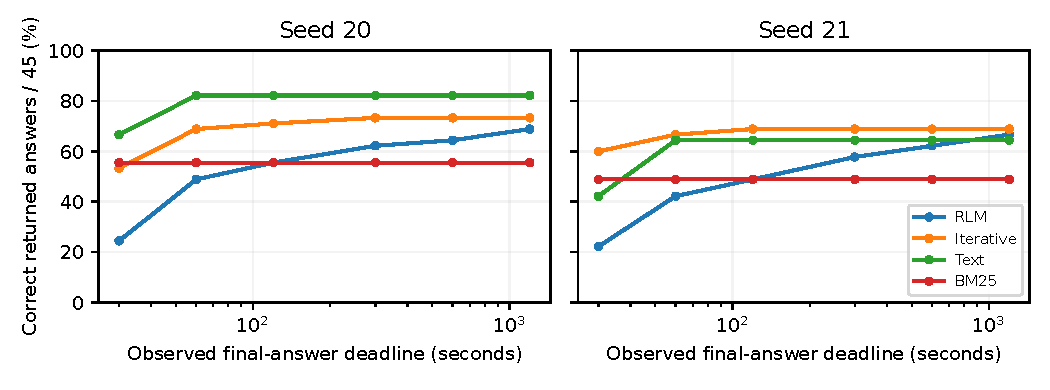
\includegraphics[width=\textwidth]{figures_expansion/observed_deadline_success.pdf}
\caption{Correct final answers returned by a given deadline on the retained runs, with all 45 queries in every denominator. The agent policy was held at its original cap: these are observed completion curves, not reruns with shorter instructed budgets. They exclude any unreturned intermediate answer and are not dollar-budget curves.}
\label{fig:observed-deadline}
\end{figure}

At 60 seconds, RLM/iterative/text/BM25 have returned 22/31/37/25 correct answers in seed 20 and 19/30/29/22 in seed 21. At 1,200 seconds the counts are 31/33/37/25 and 30/31/29/22. Longer allowed waiting reveals more correct RLM answers in these stored executions, while the relative ordering remains task- and rollout-specific. No confidence claim about fresh deployments is inferred from the curves alone.

\paragraph{Question-parser audit.}
The unchanged question parser was replayed using only the question string; the stored benchmark task and answer-type fields were used solely for checking agreement afterward. Both fields match on 150/150 SU-150 cases (73 context windows), 45/45 CD-45 cases (32 windows) and 45/45 VC-45 cases (20 windows), and every replay matches its original stored parser output. This repairs incomplete reporting of a check already represented in the stored outputs. It does not add new data or establish robustness to arbitrary paraphrases. In particular, selecting the correct task and answer type does not guarantee correct local labels, subset extraction, tie handling or the final answer.

The replay script writes per-case parser decisions, paired contrasts, exact McNemar tests with within-rollout Holm adjustment, selection decompositions, deadline counts and source hashes. Missing successful-output judgments, duplicate route/query cells and mismatched query IDs fail validation. All figures derive from the same analysis artifact.
